\documentclass[10pt]{article}

% Idioma y codificación
\usepackage[utf8]{inputenc}
\usepackage[spanish]{babel}

% Márgenes
\usepackage{geometry}
\geometry{top=2.5cm, bottom=2.5cm, left=2.5cm, right=2.5cm}

% Gráficos
\usepackage{graphicx}
\usepackage{graphics}
\usepackage{wrapfig}
\usepackage{float}

% Listings para código
\usepackage{listings}
\usepackage{xcolor}
\usepackage{caption}
\usepackage{capt-of}
\lstdefinestyle{terminal}{
	backgroundcolor=\color{gray!10},
	basicstyle=\ttfamily\small,
	keywordstyle=\color{blue},
	commentstyle=\color{gray},
	frame=single,
	columns=fullflexible,
	morecomment=[l]{//}
}
\usepackage{listings}
\lstset{
	inputencoding=utf8,
	extendedchars=true,
	literate={á}{{\'a}}1 {é}{{\'e}}1 {í}{{\'i}}1 {ó}{{\'o}}1 {ú}{{\'u}}1 {ñ}{{\~n}}1
}

% Hipervínculos
\usepackage[hidelinks]{hyperref}
\hypersetup{
	colorlinks=true,
	linkcolor=blue,
	filecolor=magenta,
	urlcolor=cyan,
}

\usepackage{url}

% Encabezados y pies de página
\usepackage{fancyhdr}
\pagestyle{fancy}
\fancyhf{}
\fancyfoot[R]{\thepage}

% Formato de títulos
\usepackage{titlesec}
\titleformat{\subsection}{\normalfont\large\bfseries}{\hspace{1em}\thesubsection}{1em}{}
\titleformat{\subsubsection}{\normalfont\normalsize\bfseries}{\hspace{2em}\thesubsubsection}{1em}{}

% Datos de la portada
\title{\textbf{Cuaderno de bitácora}}
\author{\textbf{\small Daniel Sanabria Salamanqués}}
\date{\today}

\makeatletter
\let\thetitle\@title
\let\theauthor\@author
\let\thedate\@date
\makeatother

\begin{document}
	
	\begin{titlepage}
		\centering
		\includegraphics[scale=0.3]{uva-3881270087.pdf}\\[0.5cm]
		\rule{\linewidth}{0.2mm}\\[0.4cm]
		{\huge\bfseries \thetitle}\\
		\rule{\linewidth}{0.2mm}\\[1.5cm]
		{\Large\bfseries Ingeniería Informática}\\[0.3cm]
		{\Large\bfseries Tecnologías de la Información}\\[1cm]
		{\Large \theauthor}\\[1.5cm]
		{\Large \thedate}
	\end{titlepage}
	
	\renewcommand{\contentsname}{Índice}
	\tableofcontents
	\clearpage
	\section{Instalación}
	
	\subsection{Clúster de Máquinas Virtuales}
	Para comenzar con la instalación, me dirijo a la página \url{matrix.inf.uva.es} e inicio sesión con mi cuenta de laboratorio de la escuela. Una vez hecho, observo que en el \verb|Datacenter| se encuentra mi máquina virtual \verb|vm3803.virtual.lab.inf.uva.es|. Al hacer doble clic, compruebo en la sección de \verb|Hardware| si está en el apartado \verb|CD/DVD| la imagen de \verb|Ubuntu Server|. Como no aparece, hago clic sobre ese apartado y con la opción \verb|Edit| que aparece en la parte superior, agrego la imagen a ese disco de la máquina.
	
	\subsection{Configuración de instalación}
	Tras esto, voy a la sección \verb|Console| para iniciar la máquina virtual y comenzar con la instalación de \verb|Ubuntu Server|. Lo primero es seleccionar el idioma para el sistema; en mi caso, escojo inglés. Después, indico que no quiero realizar la actualización para obtener \verb|Ubuntu Server 25.04|. Luego, para la configuración del teclado, selecciono el teclado español, debido a que mi teclado necesita esa configuración. En la siguiente pantalla, escojo que la instalación base será \verb|Ubuntu Server| por defecto y sin opciones adicionales. En la configuración de red, no modifico ningún valor ni agrego ningún \verb|proxy|. En cuanto al almacenamiento, indico que para la instalación use todo el disco y que no lo monte como un grupo \verb|LVM|. Después de confirmar la configuración del almacenamiento, relleno en la siguiente pantalla los datos de mi perfil:
	\begin{itemize}
		\item \textbf{Nombre}: Daniel
		\item \textbf{Nombre de servidor}: vm3803
		\item \textbf{Username}: dansana
	\end{itemize}
	Para la configuración de la conexión SSH, selecciono la opción de que se instale \verb|OpenSSH|. Para terminar, no agrego ninguna \verb|snap| al sistema y después de seleccionar \verb|Done|, dejo que se termine la instalación con la configuración seleccionada. Tras unos minutos, la instalación termina y reinicio el sistema.\\\\
	Una vez que ha arrancado, inicio sesión con el usuario y la contraseña que he creado y, acto seguido, procedo a purgar ciertas aplicaciones que no son necesarias.
	
	\subsection{Reconocimiento del entorno}
	Nos piden realizar un reconocimiento del entorno para conocer acerca del sistema que hemos instalado, además de saber cómo funciona la máquina virtual en la página \url{matrix.inf.uva.es}:
	\begin{itemize}
		\item \textbf{Version Kernel Linux}: El comando \verb|cat /proc/version|, nos devuelve la información acerca del Linux instalado. En este caso, se trata de un Linux con la versión el kernel 6.8.0-79-generic. El funcionamiento del comando es mostrar lo que contiene el archivo \verb|version| dentro de \verb|proc|, que se trata del sistema de ficheros.
		\item \textbf{Particiones}: Con el comando \verb|df -h|, se obtiene las particiones montadas. En este caso, tenemos las siguientes particiones:
		\begin{itemize}
			\item \textit{/dev/sda1}: Montada en el directorio \verb|/boot/efi| y es la encargada de el arranque del sistema. 
			\item \textit{/dev/sda2}: Montada en el directorio raíz \verb|/|, dedicada al resto de sistema.
		\end{itemize}
		\item \textbf{Espacio libre}: Con el mismo comando que el punto anterior, se puede ver que hay varias columnas dedicadas al almacenamiento de cada partición:
		\begin{itemize}
			\item \textit{/dev/sda1}: Con \verb|1.1G| en total, solo se ha usado el 1\%, es decir, \verb|6.2M| se ha utilizado y se encuentran disponibles \verb|1.1G| para usar.
			\item \textit{/dev/sda2}: Con \verb|58G| en total, solo se ha usado el 12\%, es decir, \verb|6.5G| se ha utilizado y se encuentran disponibles \verb|49G| para usar.
		\end{itemize}
		\item \textbf{Cerrar sesión}: Cuando se ha iniciado sesión y queremos cerrar esa misma sesión, simplemente tenemos que escribir el comando \verb|logout| y el sistema cerrará la sesión.
		\item \textbf{Apagar la máquina}: Desde la consola del sistema, mediante el comando \verb|shutdown -h| se le enviará una señal al sistema para apagar la máquina.
		\item \textbf{Reiniciar la máquina}: Para el reinicio, se emplea el comando \verb|reboot|.
		\item \textbf{Controles de la consola de la máquina virtual}: Se pide usar los controles que aparecen en la parte superior:
		\begin{enumerate}
			\item Cuando la máquina esté encendida, nos indican apagar la máquina con \verb|Stop|. Esto obligará a la máquina a hacer un apagado forzado.
			\item Después de volver a encender, nos piden restear la máquina mediante la opción \verb|Reset|. Funciona igual que escribir el comando \verb|reboot|.
			\item Por último, será apagar de nuevo la máquina pero con la opción \verb|Shutdown| que será lo mismo que escribir el comando \verb|shutdown -h|.
		\end{enumerate}
	\end{itemize}
	
	\subsection{Acceso remoto vía ssh}
	Se nos indica que el sistema ya tiene instalado y activado el servicio de conexión segura \verb|sshd| (que previamente hemos configurado en la configuración de la instalación) y para comprobar que funciona correctamente, me conectaré desde \verb|Jair| a esta máquina, usando la red de la UVa. Aquí se muestra una captura del proceso:
	\begin{figure}[H]
		\setlength{\abovecaptionskip}{0cm}
		\setlength{\belowcaptionskip}{0cm}
		\centering
		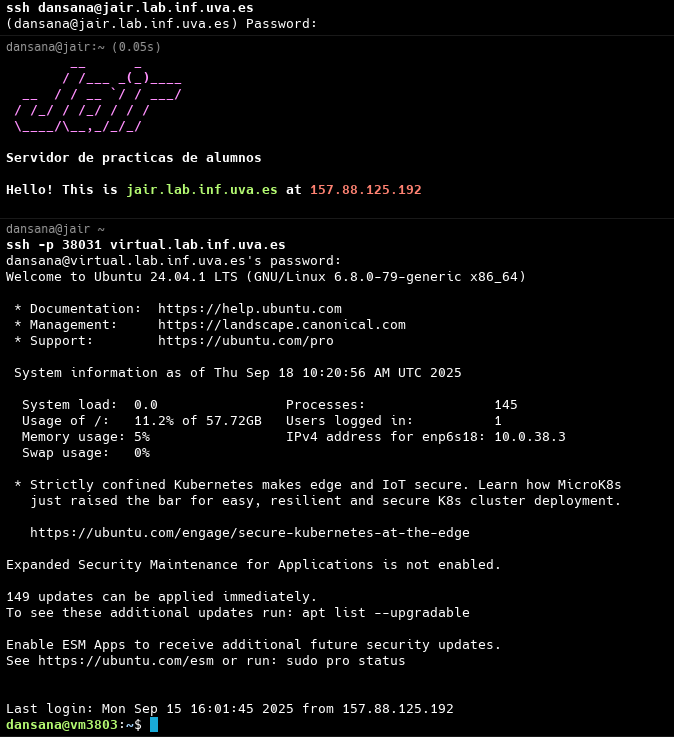
\includegraphics[width=0.6\linewidth]{Recursos/ssh.png}
		\label{fig:datos}
	\end{figure}
	
	\subsection{Activar cuenta root}
	Lo siguiente que se indica es activar la cuenta \verb|root| cambiando su contraseña mediante \verb|sudo passwd root| e indicando una clave para ese usuario y así poder acceder a la consola directamente como \verb|root|, ya que por defecto no trae ninguna contraseña y puede ser una brecha de seguridad.
	
	\subsection{Administración del disco}
	Se pide obtener información sobre las particiones lógicas y física de nuestra máquina virtual, con ayuda de los comandos que se explican en las transparencias. 
	Y para saber el sistema de ficheros que se está utilizando, tendremos que hacer un \verb|cat| al fichero \verb|/etc/fstab|, que contiene las informaciones que conciernen al montaje de las particiones que hay en el sistema.
	\begin{figure}[H]
		\centering
		\begin{minipage}{0.5\textwidth}
			\centering
			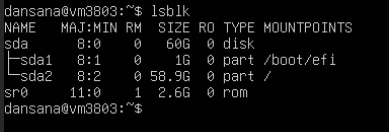
\includegraphics[width=\linewidth]{Recursos/particiones.png}
		\end{minipage}\hfill
		\begin{minipage}{0.45\textwidth}
			\begin{itemize}
				\item \textbf{Dispositivos}: Tal y como se muestra en la imagen, solo tenemos un dispositivo de almacenamiento \verb|sda| con una capacidad de 60G. El otro dispositivo que existe es el CD de instalación de \verb|Ubuntu Server| que ocupa 2.6G.
			\end{itemize}
		\end{minipage}
	\end{figure}
	
	\begin{figure}[H]
		\centering
		\begin{minipage}{0.5\textwidth}
			\centering
			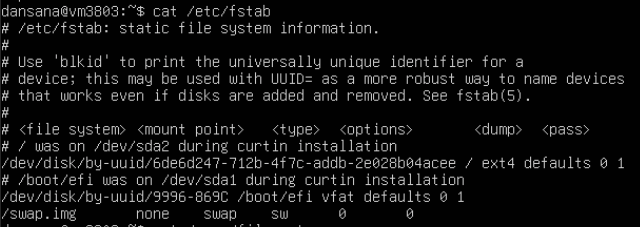
\includegraphics[width=\linewidth]{Recursos/fstab.png}
		\end{minipage}\hfill
		\begin{minipage}{0.45\textwidth}
			\begin{itemize}
				\item \textbf{Particiones}: Existen dos particiones en el disco \verb|sda|:
				\begin{itemize}
					\item \textit{sda1}: Con un tamaño de 1G y montado en el directorio \verb|/boot/efi|, es la encargada de almacenar las herramientas de arranque del sistema que serán lanzadas por el firmware UEFI. Emplea el sistema de ficheros \verb|vfat|.
					\item \textit{sda2}: Partición principal, anclado en el directorio \verb|/|, con el tamaño restante del disco para almacenar todas las aplicaciones y ficheros del sistema operativo y del usuario. Emplea el sistema de ficheros \verb|ext4|.
				\end{itemize}
			\end{itemize}
		\end{minipage}
	\end{figure}
	
	Después, se nos exige investigar el fichero \verb|/proc/filesystems| donde se ubican los sistemas de ficheros que es capaz de entender el sistema.
	\begin{figure}[H]
		\centering
		\begin{minipage}{0.28\textwidth}
			\centering
			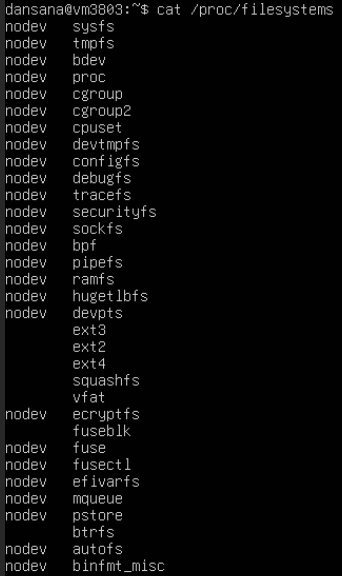
\includegraphics[width=\linewidth]{Recursos/filesystems.png}
		\end{minipage}\hfill
		\begin{minipage}{0.7\textwidth}
			\begin{itemize}
				\item Se muestra dos columnas donde en la izquierda se indica si se requiere un dispositivo de bloque asociado al sistema de fichero que se muestra en la columna de la derecha.
				\item Por ejemplo, para los sistemas de ficheros \verb|ext2, ext3 o ext4| no se indica el valor \verb|nodev|, por lo que es necesario usar un dispositivo físico para usar ese sistema de fichero. Pero, para \verb|tmpfs o proc|, no es necesario tener un dispositivo físico.
			\end{itemize}
		\end{minipage}
	\end{figure}
	
	\subsubsection{Loop} \label{loop}
	Después, creamos un sistema de archivos o fichero dentro de un fichero nuevo:
	\begin{enumerate}
		\item Creamos el fichero mediante el comando \verb|dd|, donde se le indica los siguientes parámetros:\\
		\verb|dd if=/dev/zero of=fichero bs=1 count=4096|
		\begin{itemize}
			\item \textbf{if}: Desde que fichero o directorio se van a leer los datos. Como vamos a crear un fichero vacío, haremos uso de \verb|/dev/zero| que se trata de un fichero especial desde el que se obtiene un flujo de cero, con el propósito de inicializar un fichero.
			\item \textbf{of}: Indicamos la ruta con el nombre del fichero creado. 
			\item \textbf{bs}: Indicamos el tamaño del bloque que se quiere leer y escribir. Para este caso, se escoge de 1 MB por comodidad.
			\item \textbf{count}: El número de bloques que se van a crear. En este caso 4096M que corresponden a los 4G.
		\end{itemize}
		\item El siguiente paso es crear el dispositivo de bloque sobre el fichero que hemos creado con el que trabajaremos para crear el sistema de ficheros, mediante el comando \verb|losetup|:
		\begin{itemize}
			\item Antes de crearlo, tenemos que ver los dispositivos \verb|loop| que están disponibles para asociarlo con el fichero. Para ello, lanzamos el comando \verb|losetup -f| y nos devuelve que el único dispositivo disponible es \verb|/dev/loop0|.
			\item Ahora lo único que tenemos que hacer es ejecutar este comando \verb|sudo losetup /dev/loop0 fichero|. Es necesario usar permisos de administrador, por lo que se lanzará el comando con \verb|sudo|.
		\end{itemize}
		\item Con el dispositivo de tipo bloque, le asignamos un sistema de fichero cualquiera con \verb|mkfs|. En mi caso, le asigno el mismo que el que tiene la partición principal: \verb|sudo mkfs.ext4 /dev/loop0|.
		\item Lo último es montar ese sistema de fichero nuevo en un directorio (\verb|/mnt| debido a que está dedicado a montar dispositivos).
		\item Para comprobar que lo hemos montado correctamente, usamos el comando \verb|lsblk| para ver todas las particiones montadas.
	\end{enumerate}
	\begin{figure}[H]
		\setlength{\abovecaptionskip}{0cm}
		\setlength{\belowcaptionskip}{0cm}
		\centering
		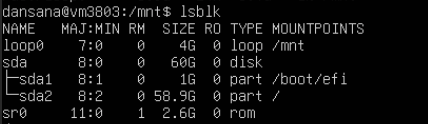
\includegraphics[width=0.6\linewidth]{Recursos/loop0.png}
		\label{fig:loop}
	\end{figure}
	
	Cuando tengamos el dispositivo de disco \verb|Loop|, nos piden administrar ñas particiones en ese dispositivo:
	\begin{itemize}
		\item Para crear una partición, haremos uso de la herramienta de \verb|fdisk|. No tendrá ningún valor específico, por lo que se deja todo por defecto.
		\item Puede ser que el kernel no pueda actualizar automáticamente la tabla de particiones al terminar, por lo que habrá que desanclar y volver anclar el \verb|Loop|.
		\item Al igual que hemos hecho con el dispositivo, habrá que formatear esa partición y asignarle un sistema de ficheros. En este caso el mismo que tiene el propio dispositivo.
		\item Después, se monta la partición con el comando \verb|mount| sobre el directorio \verb|/mnt| y se comprueba lanzando un \verb|df -h|. Tras esto, se desmonta con \verb|umount|.
		\item Ahora nos piden un resumen acerca de la función de los ficheros \verb|/etc/fstab| y \verb|/etc/mtab|:
		\begin{itemize}
			\item \textbf{/etc/fstab}: Es un fichero de configuración estático que define qué sistemas de archivos hay en el sistema y cómo deben montarse. La máquina lo consulta durante el arranque para montar automáticamente discos, particiones o sistemas de ficheros de red.
			\item \textbf{/etc/mtab}: Es un fichero dinámico, generado por el sistema, que refleja qué sistemas de ficheros están montados en este momento. En sistemas modernos, muchas veces /etc/mtab es un enlace simbólico a /proc/self/mounts, que cumple la misma función.
		\end{itemize}
		\item Por último, nos indican eliminar la partición existente en \verb|loop0| y crear varias particiones primarias y extendidas o lógicas. Además, cada partición tiene que tener un sistema de ficheros independiente. Este sería el esquema resultante:
		\begin{figure}[H]
			\centering
			\begin{minipage}{0.48\textwidth}
				\centering
				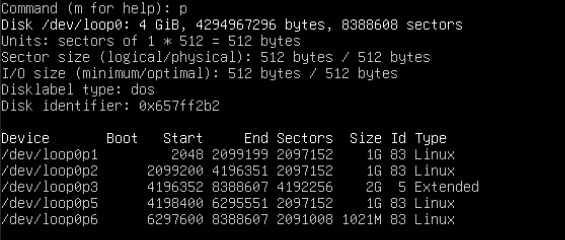
\includegraphics[width=\linewidth]{Recursos/particiones1.png}
			\end{minipage}\hfill
			\begin{minipage}{0.48\textwidth}
				\centering
				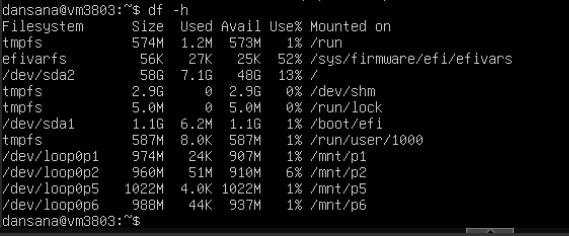
\includegraphics[width=\linewidth]{Recursos/particiones2.png}
			\end{minipage}
		\end{figure}
	\end{itemize}
	
	\subsubsection{LVM}
	Llegados a este punto, se requiere volver a destruir las particiones existentes para crear y administrar volúmenes lógicos (LVM).
	\begin{enumerate}
		\item Primero, modificamos la etiqueta de cada partición para marcar que es de tipo \verb|Linux LVM|. Desde la herramienta de \verb|fdisk|, seleccionamos cada partición del dispositivo \verb|loop0| y con la opción \verb|t|, escogemos el número 44 (en este caso que usamos una tabla de particiones de tipo \verb|GPT|).
		\item Después, creamos el volumen físico en cada partición con \verb|pvcreate|:
		\begin{figure}[H]
			\setlength{\abovecaptionskip}{0cm}
			\setlength{\belowcaptionskip}{0cm}
			\centering
			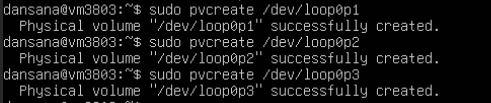
\includegraphics[width=0.6\linewidth]{Recursos/pvcreate.png}
		\end{figure}
		\item Lo siguiente, es crear un grupo de volúmenes físicos, con \verb|vgcreate|, donde agregamos los que hemos creado:
		\begin{figure}[H]
			\setlength{\abovecaptionskip}{0cm}
			\setlength{\belowcaptionskip}{0cm}
			\centering
			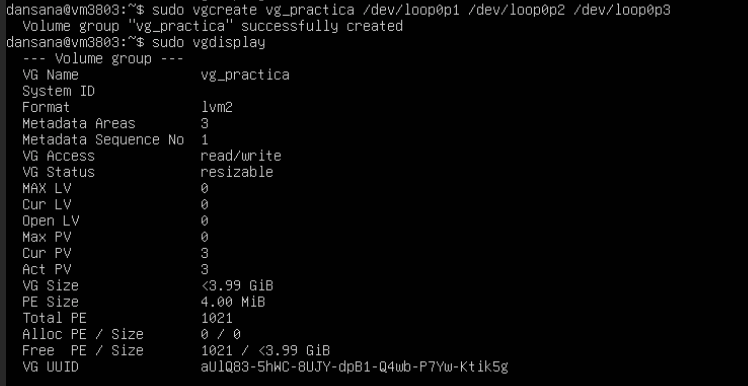
\includegraphics[width=0.6\linewidth]{Recursos/vgcreate.png}
		\end{figure}
		\clearpage
		\item Por último, creamos un par de volúmenes lógicos, con \verb|lvcreate|, sobre ese grupo que hemos creado en el punto anterior para después montarlo en el sistema:
		\begin{figure}[H]
			\setlength{\abovecaptionskip}{0cm}
			\setlength{\belowcaptionskip}{0cm}
			\centering
			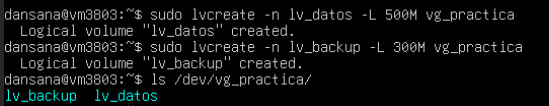
\includegraphics[width=0.6\linewidth]{Recursos/lvcreate.png}
		\end{figure}
		\item Una vez ya tenemos los volúmenes lógicos, los formateamos ambos para asignarles una estructura de directorios y los montamos en el directorio \verb|/mnt| para comprobar que se ha creado de forma correcta:
		\begin{figure}[H]
			\setlength{\abovecaptionskip}{0cm}
			\setlength{\belowcaptionskip}{0cm}
			\centering
			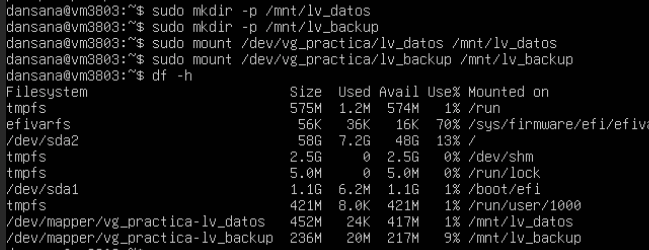
\includegraphics[width=0.6\linewidth]{Recursos/mountLVM.png}
		\end{figure}
		\item Para acabar con este apartado, retornamos el sistema a su estado anterior desmontando y eliminando los volúmenes: 
		\begin{figure}[H]
			\setlength{\abovecaptionskip}{0cm}
			\setlength{\belowcaptionskip}{0cm}
			\centering
			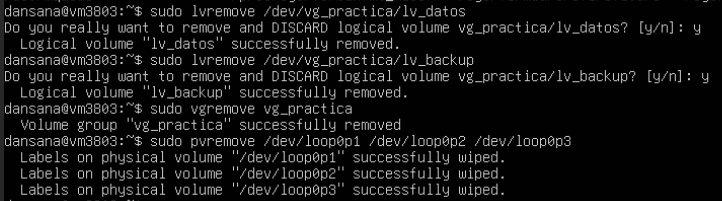
\includegraphics[width=0.6\linewidth]{Recursos/removeLVM.png}
		\end{figure}
	\end{enumerate}
	
	\subsection{Administración de almacenamiento}
	\subsubsection{RAID 5}
	Lo último que vamos a hacer antes de realizar una nueva instalación es crear y administrar un \verb|RAID 5| mediante software:
	\begin{enumerate}
		\item Lo primero es crear 3 nuevos dispositivos \verb|loop| de la misma manera que lo hemos hecho en el apartado \hyperref[sec:loop]{Loop}:
		\begin{figure}[H]
			\setlength{\abovecaptionskip}{0cm}
			\setlength{\belowcaptionskip}{0cm}
			\centering
			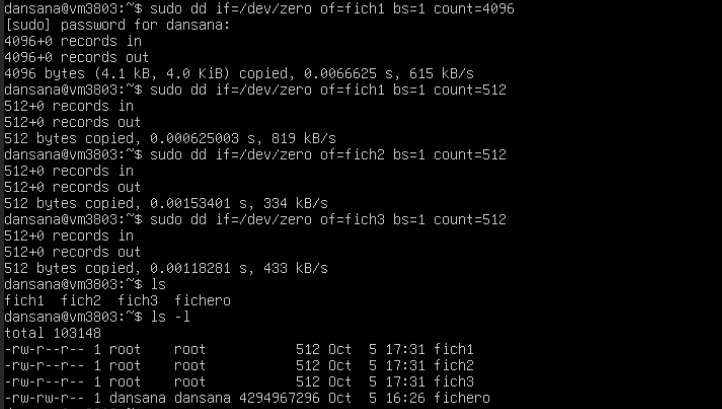
\includegraphics[width=0.5\linewidth]{Recursos/fichRAID.png}
		\end{figure}
		Y después asociarlo a 3 dispositivos \verb|loop|:
		\begin{figure}[H]
			\setlength{\abovecaptionskip}{0cm}
			\setlength{\belowcaptionskip}{0cm}
			\centering
			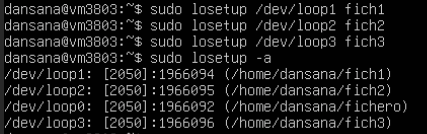
\includegraphics[width=0.5\linewidth]{Recursos/loopRAID.png}
		\end{figure}
		\item Consultando el manual para crear el dispositivo \verb|RAID|, tenemos que seleccionar el modo \verb|Create|, con las opciones de:
		\begin{itemize}
			\item \verb|level|: Indicando el tipo de \verb|RAID|.
			\item \verb|raid-devices|: Número de dispositivos que usaremos.
		\end{itemize}
		\begin{figure}[H]
			\setlength{\abovecaptionskip}{0cm}
			\setlength{\belowcaptionskip}{0cm}
			\centering
			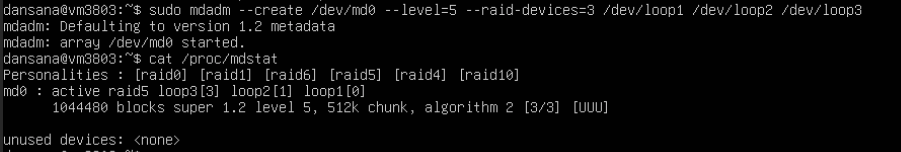
\includegraphics[width=0.6\linewidth]{Recursos/createRAID.png}
		\end{figure}
		\item Ahora repetimos el mismo procedimiento que con el resto de dispositivos de almacenamientos para formatearlos y darle un sistema de ficheros y montarlo:
		\begin{figure}[H]
			\setlength{\abovecaptionskip}{0cm}
			\setlength{\belowcaptionskip}{0cm}
			\centering
			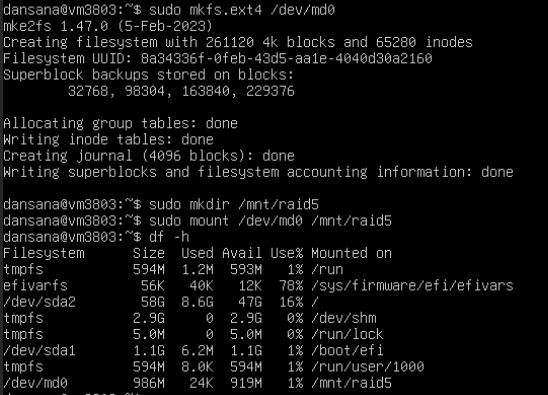
\includegraphics[width=0.6\linewidth]{Recursos/mountRAID.png}
		\end{figure}
	\end{enumerate}
	Para comprobar que hemos configurado correctamente el disco, ejecutamos el comando \\ \verb|echo “Voy a destruir el disco!!!!” > fichero.img| donde \verb|fichero.img| es uno de los ficheros que da soporte al \verb|RAID| para hacerlo fallar y ver que sigue funcionando. Al lanzarlo, veo que no se destruye el disco y sigue activo, debido a que el fichero no es el disco como tal, por lo que no pasa nada. 
	
	\subsection{Nueva instalación personalizada}
	Hasta ahora hemos trabajo con una configuración "por defecto" sobre la administración del disco de la máquina, teniendo únicamente dos particiones: \verb|/boot/efi| empleada para el arranque del sistema y \verb|/| para el resto de archivos del equipo. En un entorno real, tenemos más particiones para minimizar posibles fallos y errores, por lo que vamos a realizar una nueva instalación con las siguientes particiones:
	\begin{itemize}
		\item \verb|/boot/efi|: Contiene los ficheros para el arranque del sistema y tiene un espacio de \verb|1.049G|, que es lo que ocupaba inicialmente y no se puede modificar. El formato que tiene es \verb|fat32|, bastante antiguo y limitado, pero compatible con muchos dispositivos.
		\item \verb|/|: Destinado a todos los ficheros para el sistema operativo y con un espacio de \verb|40G| para que no haya problemas a la hora de agregar elementos al sistema.
		\item \verb|swap|: Con un espacio de \verb|1.448G|, solo actúa en caso de que la memoria RAM se quede sin espacio.
		\item \verb|/home|: Dedicada al espacio personal del usuario que ocupa el resto del espacio restante del disco.
	\end{itemize}
	\begin{figure}[H]
		\setlength{\abovecaptionskip}{0cm}
		\setlength{\belowcaptionskip}{0cm}
		\centering
		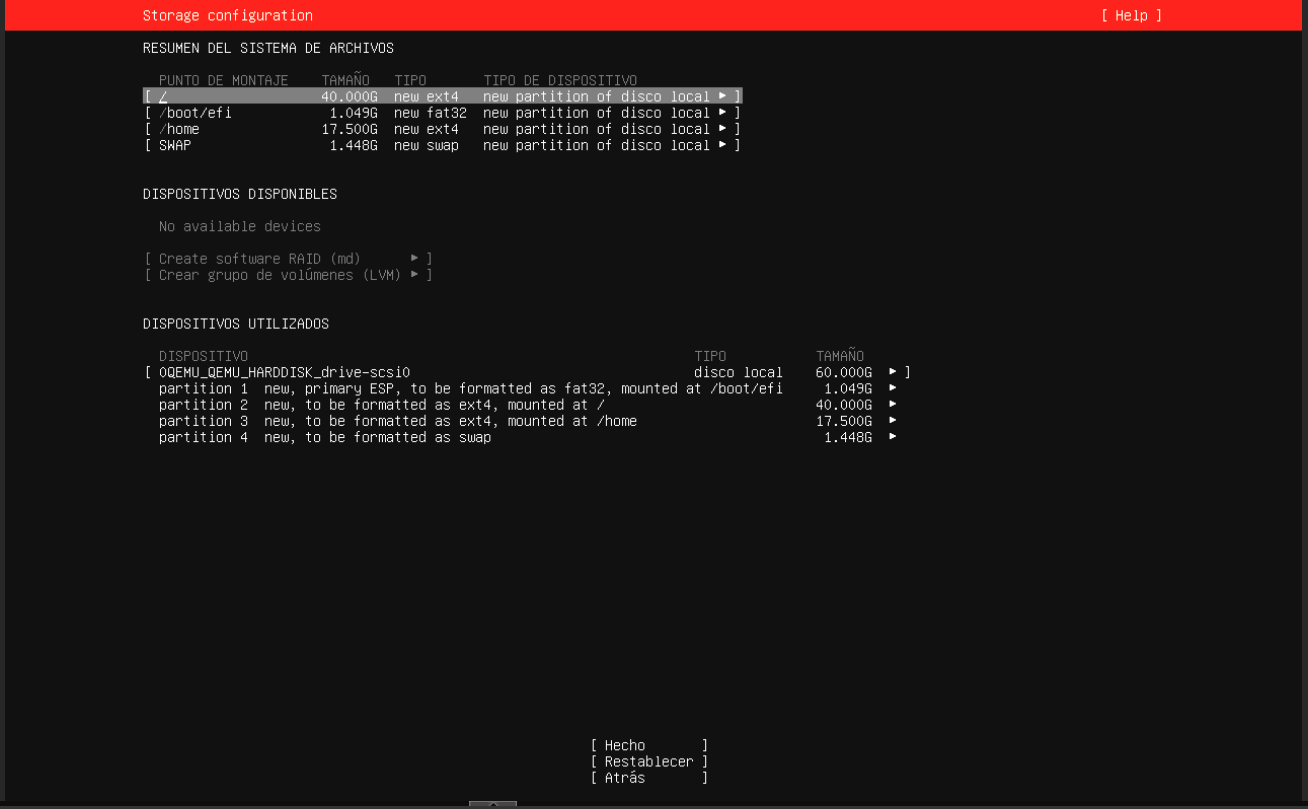
\includegraphics[width=0.6\linewidth]{Recursos/nuevaInstalacion.png}
	\end{figure}
	
	\subsection{Trabajo No Presencial}
	\begin{itemize}
		\item \textbf{Administración de discos – particiones}: 
		\begin{itemize}
			\item Los discos duros o dispositivos de bloques, se dividen en unidades lógicas llamadas \textit{particiones}.\cite{Discos}
			\item Una partición sirven organizan y almacenan el sistema operativo, las aplicaciones y los archivos personales. Existen diferentes esquemas de particiones para la distribución de particiones en un disco, como MBR o GPT.
			\item Cada partición se representa como un archivo en el sistema de archivos de Linux y se encuentra ubicada en el directorio \verb|/dev|.
		\end{itemize}
		\item \textbf{Sistemas de archivos}: 
		\begin{itemize}
			\item Se organizan en una estructura jerárquica, de tipo árbol. El nivel más alto del sistema de ficheros es / o directorio raíz. Todos los demás ficheros y directorios están bajo el directorio raíz.\cite{Archivos}
			\item Por debajo del directorio raíz (/) hay un importante grupo de directorios común a la mayoría de las distribuciones de GNU/Linux: \verb|/bin, /boot, /etc/, /opt, etc|.
		\end{itemize}
		\item \textbf{Actualización de un sistema operativo previamente instalado}:
		\begin{itemize}
			\item En el caso de nuestra máquina virtual, estamos trabajando con \verb|Ubuntu| que pertenece al grupo de distribuciones \verb|Debian|, por lo que para actualizar el sistema operativo una vez instalado se hará uso de la herramienta \verb|apt|.
			\item \verb|apt| nos proporciona un sistema de gestión de paquetes donde maneja automáticamente las dependencias para la instalación de esos paquetes. Requiere de privilegios administrativos.\cite{Actualizar}
			\item Para las actualizaciones será necesario usar los comandos \verb|sudo apt update| y \verb|sudo apt upgrade|.
		\end{itemize}
		\item \textbf{Identificación discos duros y particiones}:
		\begin{itemize}
			\item En Linux, los dispositivos se representan dentro del directorio \verb|/dev| y se identifican como dispositivos de bloques (\verb|sda, sdb, sdc, etc.| o \verb|nvme0n1, nvme0n2, nvme0n3, etc.|).
			\item Además, las particiones, tal y como se mencionaba en el primer apartado, son unidades lógicas de estos dispositivos y se identifican numerándose en orden seguido del nombre del dispositivo (\verb|sda1, sda2, sda3, etc.| o \verb|nvme0n1p1, nvme0n1p2, nvme0n1p3, etc.|).\cite{Discos}
			\item También, cada partición puede tener un \verb|UUID| único, que no cambia aunque el disco se conecte en distinto orden.
		\end{itemize}
		\item \textbf{RAID}: 
		\begin{itemize}
			\item \verb|RAID| o Redundant Array of Independent Disks hace referencia a un sistema de almacenamiento de datos que utiliza múltiples discos duros, entre las cuales se distribuyen o replican los datos. \cite{RAID}
			\item Estas son las principales configuraciones de \verb|RAID|:
			\begin{itemize}
				\item \textbf{RAID 0}: Distribuye los datos equitativamente entre dos o más discos sin información de paridad que proporcione redundancia. No tiene tolerancia a fallos, si falla un disco, lo pierdes todo.
				\item \textbf{RAID 1}: Crea una copia exacta de un conjunto de datos en dos o más discos. Puede fallar solo un disco para no perder todos los datos.
				\item \textbf{RAID 5}: División de datos a nivel de bloques que distribuye la información de paridad entre todos los discos miembros del conjunto. Esta variante de \verb|RAID| ha logrado popularidad gracias a su bajo coste de redundancia. Puede tolerar 1 disco defectuoso; reconstrucción en curso mientras funciona.
				\item \textbf{RAID 6}: amplía el nivel RAID 5 añadiendo otro bloque de paridad, por lo que divide los datos a nivel de bloques y distribuye los dos bloques de paridad entre todos los miembros del conjunto. Puede tolerar 2 discos defectuosos; más seguro que RAID 5 en entornos con discos grandes.
			\end{itemize}
		\end{itemize}
	\end{itemize}
	
	\clearpage
	\bibliographystyle{plain}
	\bibliography{bibliografia}
\end{document}